\emph{Component and Composite:}
A component assurance is an assurance that describes a single AIA capability (or one aspect of an AIA model/process for a capability), and targets one or more trust dimension targets.  Component assurances are perhaps the most well researched in the existing literature. A component assurance might include displaying the confidence of a classification prediction, or visualizing a model. A composite assurance is the combination of more than one component assurance into a single assurance. 
%Composite assurances are assurances that are built of several components. 
A notable example is the machine self-confidence work by \citet{Aitken2016-cv} which notionally combines five component assurances into a single composite assurance that a non-expert AIA user can easily and interpret. 

Figure \ref{fig:assurance_mapping} illustrates the concepts of component and composite assurances. Some open questions here are: how can component assurances generally be combined to create a composite one? Also, to what extent can component and composite assurances be used in concert to provide assurances for users of differing expertise? And are the effects of a composite assurance equal to the sum of its components?

\begin{figure}[!htbp]
    \centering
    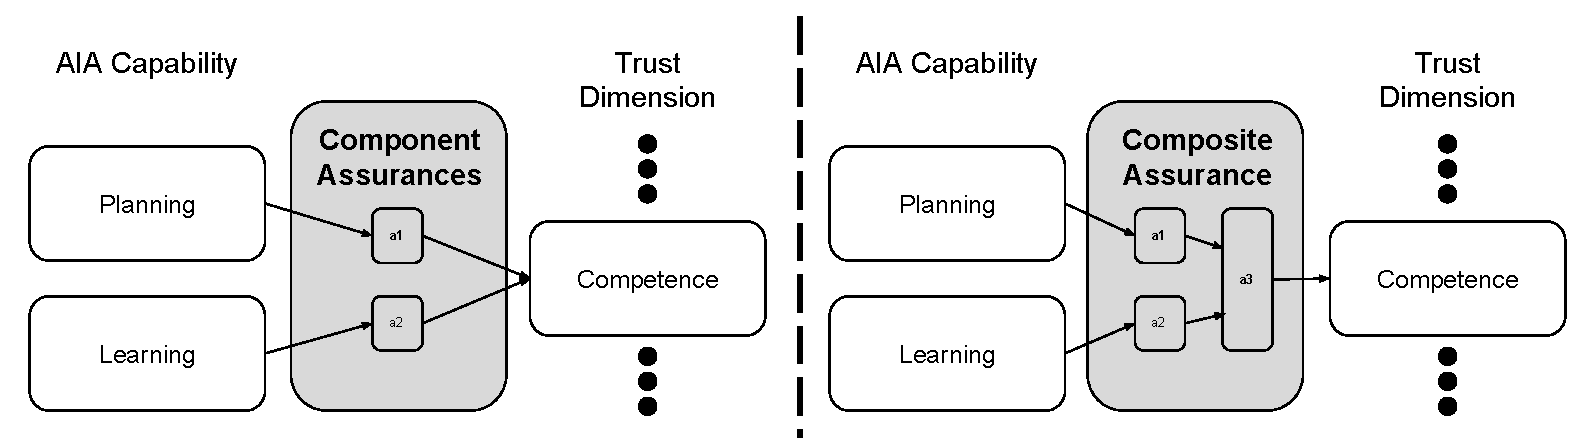
\includegraphics[width=0.7\textwidth]{Figures/Assurance_component_composite.pdf}
    \caption{%Figure illustrating the difference between component and composite assurances. The existence of multiple assurances does not imply a composite assurance, rather the combination of multiple component assurances into a single assurance constitutes a composite assurance. On the left there are two component assurances $a1$ and $a2$, whereas on the right only $a3$ affects the trust dimension.
    Component vs. composite assurances: the combination of multiple component assurances into a single assurance is a composite assurance. On the left are two component assurances $a1$ and $a2$; on the right only $a3$ affects the trust dimension.}
    \label{fig:assurance_mapping}
\end{figure}
